\begin{figure}[htb]
\centering
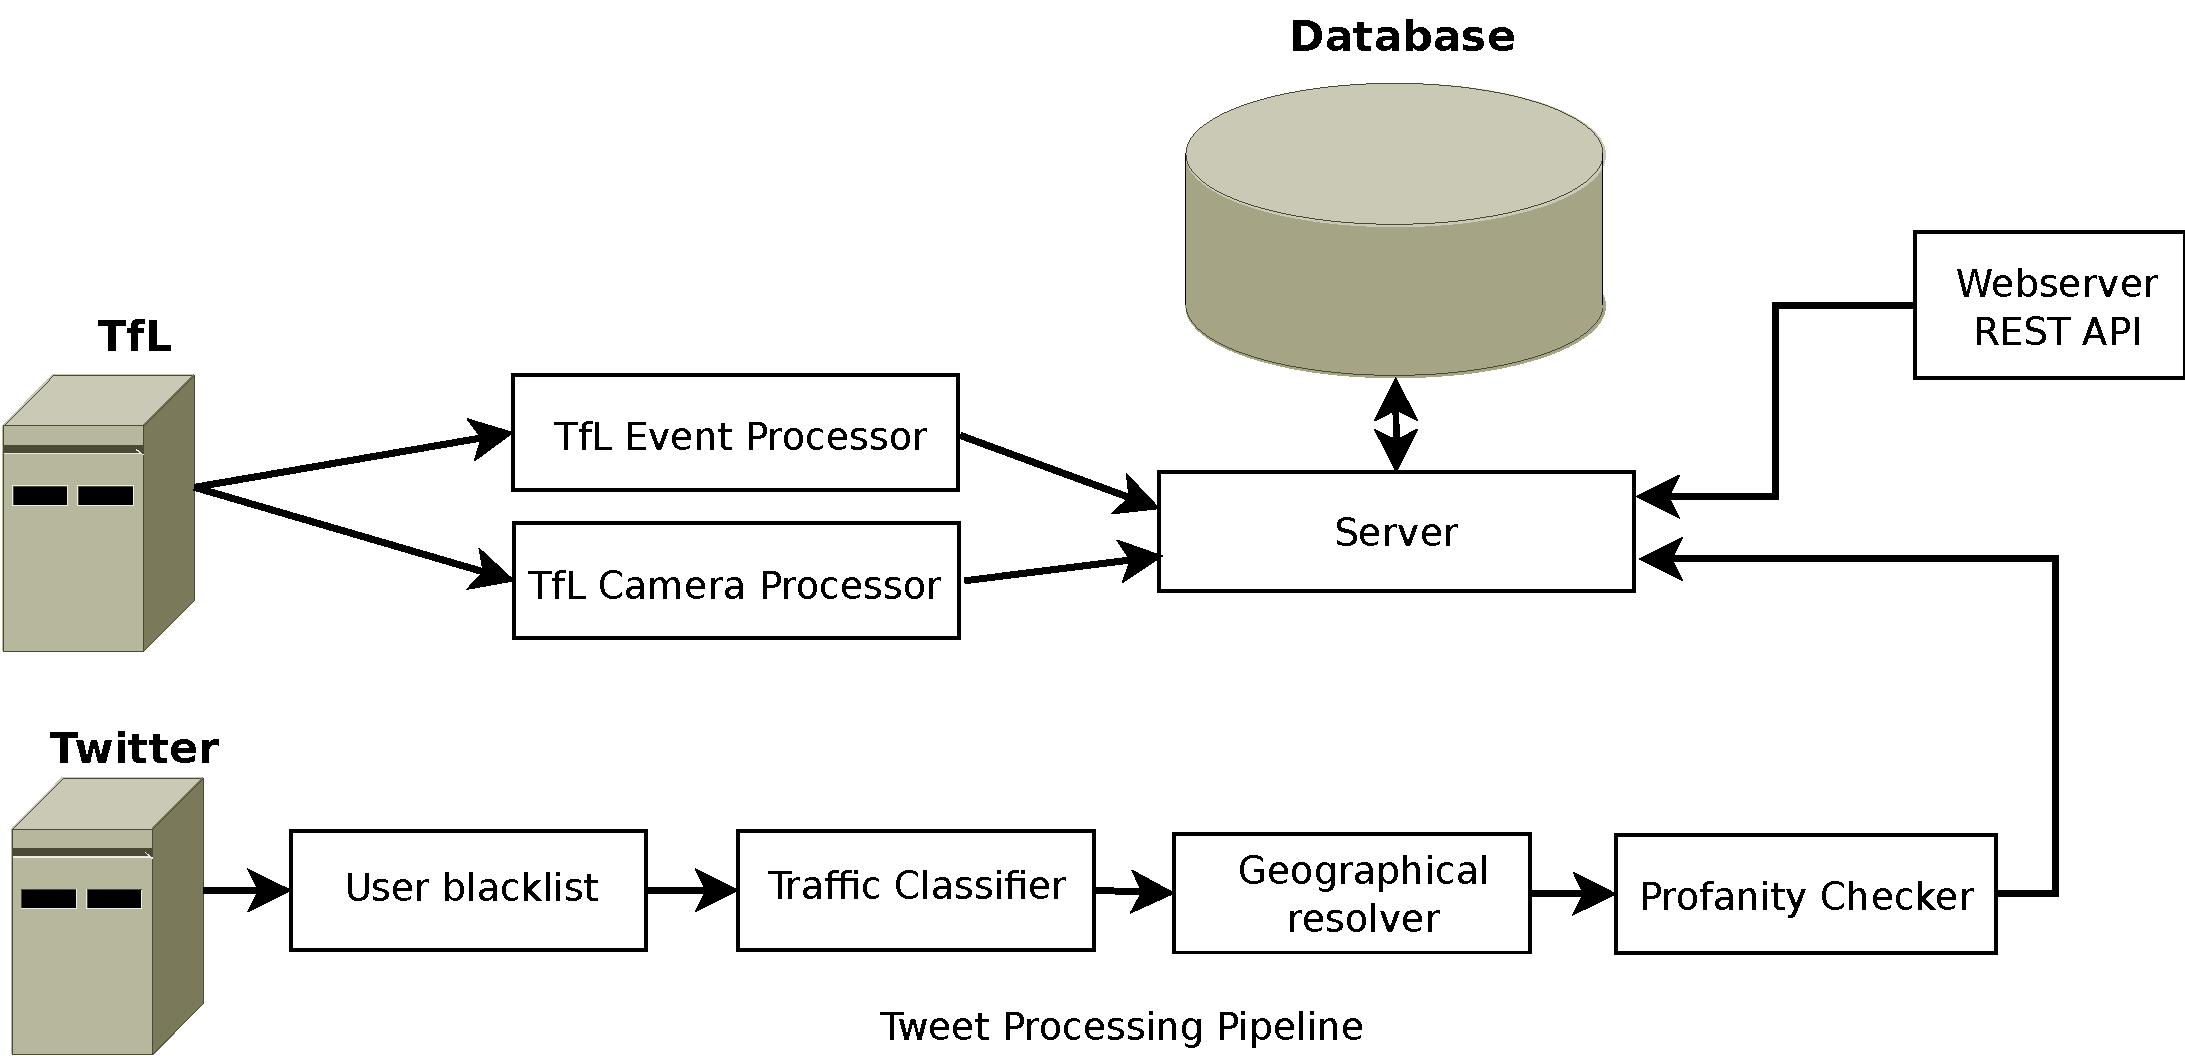
\includegraphics[width=1\textwidth]{images/design/server/server.pdf}
\caption{Server Design}
\label{fig:server_design}
\end{figure}

\subsubsection{Data acquisition}
The sources that we collect data from are Transport for London (TfL) and Twitter.

The TfL website provides different types of data feeds that can be used to obtain information relevant to traffic. 
One of the TfL data feeds we use is the "live traffic disruptions". This provides information about traffic disruption events in the area of London. This information contains details about the severity of the event, the type (e.g. road works, signal failure, accident), the location and an estimated time for the event's end.

To provide a more complete view around the area of the event we also store the "live traffic camera images" feed from TfL. This provides urls to pictures taken by traffic cameras within the last 15 minutes as well as the location of the camera and the timestamp when the picture was taken.

These feeds are returned in XML format and need to be parsed before we store them in the database. To achieve this, we use the xml.dom.minidom python module. This can parse the XML file to a Document Object Model (DOM). A DOM tree can be accessed by using functions to call each field of the XML object that was used to create it.

Because a TfL traffic event's position is returned as a point in British national grid coordinates, we first transform them to longitude and latitude coordinates before storing them in the database. This is done using a python module that implements the algorithm given in the ordnance survey guide.\cite{grid2lonlat_alg} \cite{grid2lonlat_impl}

For Twitter we defined the area around London that we are interested to collect tweets from. In addition to this, we used a search query with the words that we want the results from Twitter to contain. This query is:  «traffic OR accident OR tailback OR gridlock OR m25 OR standstill OR road OR street OR stuck OR car OR bus OR delay».

In contrast to the TfL, the Twitter data are returned in a JSON format. For this reason, we used the python-twitter API which saves the JSON information into classes and variables that can then be easily accessed. Before storing the tweets to the database each of them passes through a processing pipeline.

First, the username of the person who sent the tweet is checked to find out if he is in the blacklist. The blacklist is a txt file we have in the server which can contain different usernames for twitter accounts from which we do not want to store tweets. The reason for this is that we can use this blacklist for traffic (or other) bots so that we only have real persons' tweets in the database. Then, we use the classifier to decide if the tweet's text is about traffic or not. The process of classification is described in the Data Analysis section. After classifing a tweet as traffic, we use a regex to find any streets or roads in its text. Finally, before storing the tweet we check a list of words that we have in a txt file to determine if they are included in the message. This is implemented for a profanity filter.

\subsubsection{Data analysis}
A big and crucial part of the project was the data analysis. Specifically for the needs of the project a sub category of the data analysis, which is called text classification, has been implemented. The text classification was necessary because the project is required the tracking of the traffic-about tweets and their presentation in the application. Moreover, the identification of the disruptions through the clustering of the tweets, is strongly depended with the recognition of the tweets as traffic or as non traffic. 

Text classification is a way to categorize documents or pieces of text. By examining the way the words are being used in a piece of text, classifiers can decide, after the training, what class label to assign to it. A binary classifier decides between two labels, such as traffic or non-traffic. The text can either be one label or the other, but not both, whereas a multi-label classifier can assign one or more labels to a piece of text. 

Two approaches for the automatic document classification exist: the supervised document classification and the unsupervised classification (clustering). The supervised classification requires a training data from the humans in order to gain the “knowledge” of the classification. The clustering doesn’t require human to have the foreknowledge of the classes, and mainly using some clustering algorithm to classify a text. The team decided to adopt the supervised classification because it’s a more stable technique and it can be used as soon as the classifier is been trained. On the other hand, the unsupervised classification has to start somewhere, and its algorithms try in iterative ways to reach a stable configuration that makes sense. Therefore it may require a large amount of time to reach this configuration, halting the rest development pipeline of the project. That’s because the classified data is required from other parts of the project. Additionally, the results of the unsupervised classification vary widely and may be completely off if the first steps are wrong.

Classification works by learning from labelled feature sets, or training data, to later classify an unlabelled text, or a feature set. A feature set is basically a key-value mapping of feature names to feature values. In the case of text classification, the feature names are usually words or blocks of words, and the values are all True. As the texts may have unknown words, and the number of possible words may be very large, words that don't occur in the text are omitted, instead of including them in a feature set with the value False.

For the project it was essential to classify the tweets that the Search API was fetching, as traffic or as non-traffic. The non-traffic tweets are being rejected while the tweets about traffic are being stored in the database, in order to be correlated with the current disruption and then presented to the application. For this purpose several classification techniques have been implemented and tested. To be more specific, the team has investigated the classification of the tweets with the methods Support Vector Machines and Naive Bayes. 

Those two algorithms have been selected cause of a number of reasons. Firstly, Naive Bayes train very quickly since it requires only a single pass on the data   to compute the normal probability density function. It also requires little storage space during both the training and classification stages: the strict minimum is the memory needed to store the prior and conditional probabilities. Additionally Naive Bayes is very transparent, as it is easily grasped by users and it provides a discrete probability for each tweet helping the ranking of the tweets. Naive Bayes is considered to have high bias, because it assumes that the dataset under consideration can be summarized by a single probability distribution and that this model is sufficient to discriminate between classes. This high bias usually generates simple, highly constrained models. On the other hand, SVM is considered to be one of the most accurate classifier when dealing with multidimensions and continuous features. However for the SVM, a large sample size is required in order to achieve its maximum prediction accuracy whereas Naïve Bayes may need a relatively small dataset.

\textbf{Naive Bayes}

Given a set of objects, each of which belongs to a known class, and each of which has a known vector of variables, the aim is to construct a rule which will allow the assigning of future objects to a class, given only the vectors of variables describing the future objects. Problems of this kind, called problems of supervised classification, are ubiquitous, and many methods for constructing such rules have been developed. One very important method is the Naive Bayes Reasoning. This is a well- established Bayesian method primarily formulated for performing classification tasks. Given its simplicity Naive Bayes models are effective classification tools that are easy to use and interpret. Naive Bayes is particularly appropriate when the dimensionality of the independent space. For the reasons given above, Naive Bayes can often outperform other more sophisticated classification methods. A variety of methods exist for modelling the conditional distributions of the inputs including normal, lognormal, gamma, and Poisson. 

This classifier has been created using the Bag of Words model and the NLTK suites of libraries. NLTK is the Natural Language Toolkit, a comprehensive Python library for natural language processing and text analytics. The group decided to use the Natural Language Toolkit because of its simplicity, consistency, extensibility and its modularity. Additionally some of the members had already experience with it and they were aware of its efficient and its good classification results. Furthermore, it was decided the usage of the Bag of Words feature extraction. Text feature extraction is the process of transforming what is essentially a list of words into a feature set that is usable by a classifier. The NLTK Naive Bayes classifier expects dictionary style feature sets, so the text should be transformed into a dictionary. The Bag of Words model is a well-known method for representing documents, which ignores the word orders. It constructs a word dictionary from all the words of an instance where every word gets the value True. An instance is a single feature set. It represents a single occurrence of a combination of features. A labelled feature set is in fact an instance with a known class label that we can use for training or evaluation.

As it has been mentioned before, for the training of the classifier it’s required a labelled data. To accomplish that, a simple script was created. This script was being executed on a temporary table on the database which was containing raw, unlabelled, tweets. During the execution it was presenting random tweets from this table and the user was able to press four buttons in order to label the tweets as traffic (personalized tweets about traffic), non-traffic, unclear and bot (tweets about traffic from official sites). After the gathering of a big amount of traffic-about tweets, the table in which the labelled tweets were being stored was used to train the classifier. However, before this data was used to train the classifier, a several linguistic normalization has been applied on the labelled text.  More details for the normalization will be described in a next section.

\textbf{Support Vector Machines}

The second supervised learning method that it was fully integrated and tested is the Support Vector Machines (SVM). This is a method that performs regression and classification tasks by constructing nonlinear decision boundaries. Because of the nature of the feature space in which these boundaries are found, Support Vector Machines can exhibit a large degree of flexibility in handling classification and regression tasks of varied complexities. There are several types of Support Vector models including linear, polynomial, RBF, and sigmoid.
In this project PyML was used to implement SVM classification. The results of
this algorithm did not show much improvement compared to Naive Bayes
classification. Also the library seems to be at an early stage which makes it
more difficult to use. Since the accuracy does not change, the use of Naive
Bayes was decided by the group.

\textbf{Normalization}

For both of the above methods a separate class has been created to be used for the tweets normalization. Normalization is the way to eliminate the low information features. Eliminating low information features gives to the model clarity by removing noisy data. Additionally it reduces the possibility to get over-fitting. By using the higher information features, the performance is increasing while the size of the model is decreasing, which results in less memory usage along with faster training and classification. This normalization was being applied on the labelled tweets before the classifier training and is continue being applied on the newly fetched tweets as well. Using this pre-processing on the tweets the accuracy of the classifier has been increased. On the following paragraphs we will present the normalization techniques which have been adopted. 

The first step was to convert the current links to a more readable way. This has been done by using a regular expression to recognize the link. After that the domain is being extracted from the url and it replaces the link itself. The next step is to replace the emoticons with a global name so they will not be deleted during the punctuation removal. That’s important because the emoticons offer useful information during the classification. For this purpose, the team has integrated a script which is responsible to find those emoticons, assign them to a group of emoticons and replace them with the name of the group. Four groups of emoticons have been created: Happy, Sad, Very Happy, Very Sad. The next step is to remove the punctuations. The team has accomplished that by creating a regular expression which represents all the possible punctuations. 

After the above linguistic transformations, the tweets are being tokenized into words. Then the unnecessary special words, like the usernames, are being removed from the tweets. Subsequently, lemmatization is being applied on the tokenized data by removing and replacing word suffixes to arrive at a common root form of the word in order to group up the common words. This method has been chosen over the stemming, because lemma is a canonical set of words, instead of the stem which in many cases is not a real world. Afterwards several stopwords have been ignored from the tweet during the classification. However, because of the natural of the tweets of being an unstructured language, the accuracy of the classifier has dropped radically. Therefore the team decided not to use the stopwords as part of the normalization. The last but not least step of the text normalization is the tracking of the bigrams collocations from the tweets. Because the bigrams are less common than most individual words, including them in the Bag of Words increases the classifier accuracy.

\textbf{Soundex}
When people are typing tweets, there are some spelling mistakes or abbreviations in them. It is difficult for server to understand the meaning of those sentences with spelling mistakes or abbreviations.This project introduce Soundex algorithm which is a phonetic algorithm for indexing names by sound, as pronounced in English. Its goal is for homophones to be encoded to the same representation so that they can be matched despite minor differences in spelling. The algorithm mainly encodes consonants; a vowel will not be encoded unless it is the first letter. That means a wrong street name will probably matches the right street name if the first letter in the street name is not typed wrongly.
In project, a 'geolookup' table which stores street address is created for looking up geolocation. When a tweet doesn't have geolocation, it will be parsed to extract street address which is used to search corresponding geolocation in 'geolookup' table. However, some addresses cannot find geolocation because there is spelling mistakes or abbreviations in it. We split street address into independent words and remove white-spaces inside. Then we encode those words using Soundex algorithm to get results and combine them into a string. This string created by Soundex algorithm is compared with other Soundex strings which is converted from street addresses in 'geolookup' table. This algorithm improves the ratio of street address matching.



\subsubsection{Storage}
For the storage of data we use a PostgreSQL database. Because of the high amount of database queries we needed to use an efficient way to store and analyze the information we acquired from the tfl feeds and twitter. For this reason, we decided to use a Geographic Information System called PostGIS. This allowed us to store geolocations (longitude and latitude) as points.

With the use of PostGIS queries to the database became easier and more efficient. The use of functions provided by PostGIS, such as ST\_DWithin to find all points around a route or a point within a radius, or ST\_Distance to find the distance between two points, made all queries simpler. In addition, the main advantage of PostGIS is that it uses generalized search trees (GiST) to index the geometries. 

A GiST like a B-tree uses key-pointer pairs. The difference with B-trees is that a GiST key is a user-defined data type. This allows different types of operations, rather than simple comparisons, such as nearest-neighbor searches and statistical approximations over large data sets. In PostGIS, the GiST is used for spatial indexing by allowing the index to use a bounding box for each geometry (e.g. line) instead of storing the whole geometry in it. Therefore, with bounding box comparison, instead of comparing geometries, functions such as ST\_DWithin are made more efficient. \cite{postgis_stdwithin}

For the project we used the following tables:
\begin{itemize}
\item Tables used by the final application
  \begin{itemize}
  \item tfl: The current tfl disruption events
  \item archive: To store old tfl disruption events for further analysis
  \item tflcameras: The current camera pictures' url
  \item tweets: To store the traffic tweets acquired from twitter
  \item geolookup: Used to store addresses with their SoundEX value and their geolocation which is acquired from Google Maps
  \item tweets\_metrics: Used to store different types of metrics for the tweets
  \end{itemize}
\item Tables used to train the classifier
  \begin{itemize}
  \item labelled\_tweets: To store manually labelled tweets as traffic or non-traffic
  \item stop\_words: Words that can be removed before data analysis
  \end{itemize}
\item Tables used by PostGIS
  \begin{itemize}
  \item geography\_columns: This is a view that shows all the columns of the database that use geography points
  \item spatial\_ref\_sys: A list of spatial reference systems and details to transform between them
  \end{itemize}
\end{itemize}

\subsubsection{Interface}

Before the actual server was implemented, the creation of a mock server api was essential. This 
provided us with the ability to seperate the work on the application and server design from the very 
beginning of the project. At this stage, the rest endpoints had to be defined in order to agree on the 
data format that was transferred between the server and the client. The next thing was creating mocked 
JSON data for responding to the requests. Such data included fixed sets of disruptions, tweets and 
cameras. 

The server is consisted of four different threads. Three of these threads are used to collect the data feeds from TfL and Twitter, as described in a previous section. The last thread is used by the REST server to receive and respond to mobile client requests. The reason for the implementation of the different threads is to achieve a fault resilient server. If one of them stops working because of an unexpected error, the remaining threads can continue to work unaffected. Furthermore, each thread uses a log file to store information about its actions and the errors it has encountered which makes debugging simpler.

The REST server can receive GET or POST requests from the mobile client. If the request was not in the correct format then the server returns a bad request (Error 400). The response to these requests is a JSON file. The different types of requests are the following:

\begin{itemize}
\item Disruption Requests
  \begin{itemize}
  \item A GET request that returns all current disruptions in an area defined by a point (longitude and latitude) and a radius.
  \item A GET request that returns all current disruptions in an area defined by 2 points that are the 2 opposite corners of a rectangle.
  \item A POST request that posts a json file of points on a route that will return all disruptions around it.
  \end{itemize}
  All these types of requests return all information of the disruptions and the cameras that are close to these events. There is also an option to return only the closest camera for each request.
\item Tweet Requests
  \begin{itemize}
  \item A GET request that returns all tweets that are around a disruption event.
  \item A GET request that returns all tweets in a area defined by a point (longitude and latitude) and a radius.
  \end{itemize}
  For both requests there is also an option to use the profanity filter for the tweets that are stored in the database.
\item Camera Requests
  \begin{itemize}
  \item A GET request that returns all cameras that are around a disruption event.
  \item A GET request that returns all cameras in a area defined by a point (longitude and latitude) and a radius.
  \end{itemize}
  These requests have an option to return only the closest camera.
\end{itemize}
